\chapter{Method}\label{chapter:first_real_chapter}

\section{Model}
Our method is based on a VAE\cite{kingma2014autoencodingvariationalbayes}.Similar to Kingma et al., we assume that the data is generated by a random process, which is dependent on the random variable \boldmath{z}. Where \boldmath{z} can be sampled from a prior distribution $p_\theta(z)$. \boldmath{x} is then generated from the conditional distribution $p_\theta(x|z)$. This results in the generative process in Eq.~\ref{eq:vae-process}. Furthermore it is assumed that the true posterior density $p_\theta(z|x) = \frac{p_\theta(x|z)p_\theta(z)}{p_\theta(x)}$ is intractable.  Kingma et al. introduce an approximation of $p_\theta(x|z)$, $q_\phi(z|x)$, also reffered to as the probabilistic encoder.
We extend this with the assumption that there exist an unique mapping $f: X \mapsto Y$, resulting in Eq.~\ref{eq:equalities}. 
\begin{subequations}
    \begin{align}
        p_\theta(x, z) & = p_\theta(x|z)p_\theta(z) \label{eq:vae-process}        \\
        p_\theta(y|z)  & = p_\theta(f(x)|z) = p_\theta(x|z) \label{eq:equalities} \\
        p_\theta(y, z) & = p_\theta(x|z)p_\theta(z)\label{eq:label-process}
    \end{align}
\end{subequations}
Taking Eq.~\ref{eq:equalities}, we can plug that into the Eq.~\ref{eq:beta-elbo}, resulting in Eq.~\ref{eq:beta-label-elbo}.
\begin{equation}
    \label{eq:beta-label-elbo}
    \mathcal{L}_{\beta-label} = \mathbb{E}_{q_{\phi}(z|x)}[\log p(y|z)] - \beta (D_{KL}(q_{\phi}(z|x) || p(z)))
\end{equation}


This results in the following three distributions we want to estimate using an neural network.
\begin{itemize}
    \item $q_\phi(z|x)$ (i.e. image encoder)
    \item $p_\theta(x|z)$ (i.e. image decoder)
    \item $p_\theta(y|z)$ (i.e. label decoder)
\end{itemize}
We will refer to the image encoder and label decoder together as VAE-Segmentation (VAES).

\subsection{Image Encoder}
The image encoder approximates the latent distribution, $p(z)$. To ensure we can train the encoder using gradient descent, we need to make sure it is fully differentiable. Thus we make use of the reparameterization trick. Using a deterministic mapping $g_\phi(\epsilon, z')$, where $\epsilon$ is an independent random variable and $g_\phi(x)$ is our (deterministic) neural network. Kingma et al. show that using this reparameterization trick, a wide range of distributions can be learned. In our case we use a Gaussian latent space. The reparameterization then becomse $z = \mu + \sigma \epsilon$, where $\mu$ and $\sigma$ are the output of our image encoder network.

\subsection{Image Decoder}
The image decoder approximates the conditional Gaussian distribution $p_\theta(x|z)$. It is used during the pretraining step to prime the image encoder with 'good' initial weights, using the traditional ($\beta$)-VAE training. The hypothesis is, that given that $x$ can be reconstructed from the learned $q_\phi(z|x)$, the learned latent space contains useful features to approximate $p_\theta(y|z)$. In Eq.~\ref{eq:beta-elbo} $log p(x|z)$ can be calculated using Eq.~\ref{eq:log_p_x_z} using a parameterized neural network.

\begin{equation}
    \begin{split}
        log p(x|z)              & = log \mathcal{N}(x; \mu, \sigma^2I) \label{eq:log_p_x_z} \\
        \text{where}~\mu,\sigma & =NN_\phi(z)
    \end{split}
\end{equation}

\subsection{Label Decoder}
The label decoder is similar to the image decoder, except that it approximates a multivariate Bernoulli distribution, instead of an Gaussian. Thus the only difference is the calculation of $log p(y|z)$, which is shown in Eq.~\ref{eq:log_p_y_z}.

\begin{subequations}
    \begin{align}
        log p(y|z)     & = \sum_{i=0}^n y_i log h_i + (1 - y_i)log(1-h_i) \label{eq:log_p_y_z} \\
        \text{where}~h & = softmax(NN_\phi(z))
    \end{align}
\end{subequations}

To improve the sharpness of the labels, additional latent variables are added from higher up the encoder, similar to HVAE. This results in the final loss Eq.~\ref{eq:beta-hvae-label-elbo}.

\begin{equation}
    \label{eq:beta-hvae-label-elbo}
    \mathcal{L}_{\beta-label} = \mathbb{E}_{q_{\phi}(z|x)}[\log p(y|z)] - \beta \sum_{i=0}^n(D_{KL}(q_{\phi}(z_i|x) || p(z_i)))
\end{equation}

\begin{figure}[h]
    \begin{minipage}{0.9\textwidth}
        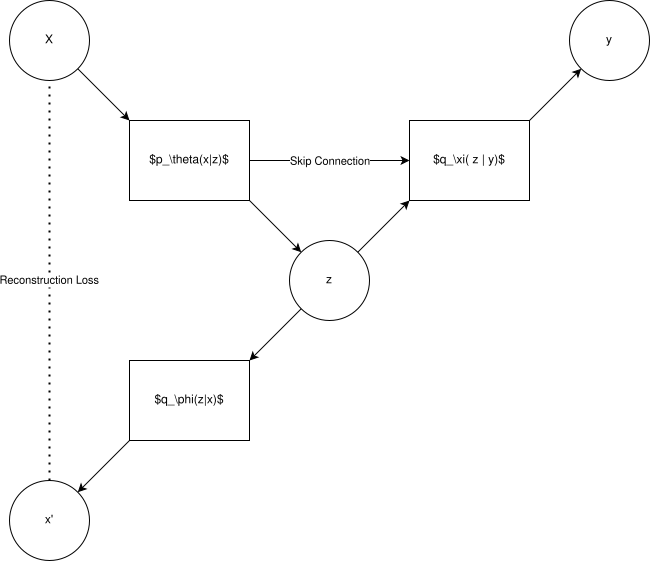
\includegraphics[width=1\textwidth]{figures/model_data_flow.png}
        \caption{The data flow of the various submodels. NOTE: I still want to make this prettier, making it more similar to \ref{fig:hvae-example}}
        \label{fig:seg-vae-schematic}
    \end{minipage}
\end{figure}

\begin{figure}
    \begin{minipage}{0.9\textwidth}
        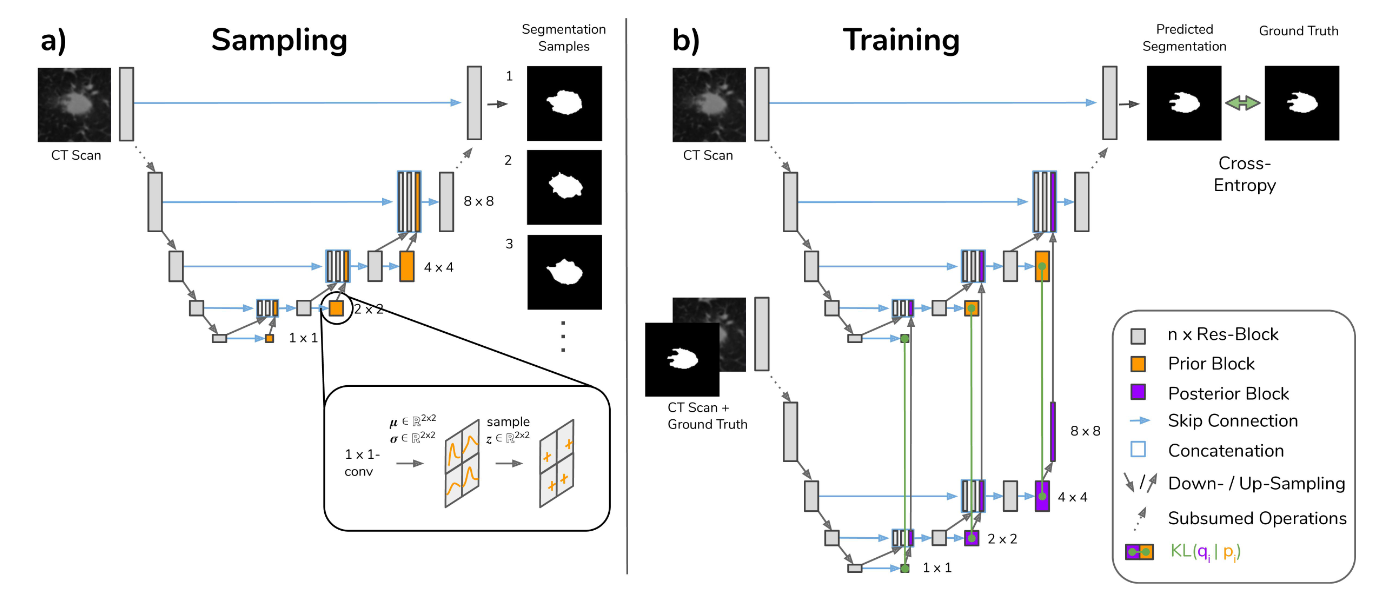
\includegraphics[width=1\textwidth]{figures/h_vae_structure.png}
        \caption{Example of the H-VAE structure. From \cite{kohl2018probabilistic}.}
        \label{fig:hvae-example}
    \end{minipage}
\end{figure}

\section{Training procedure}
First, a $\beta$-vae is trained on the full training dataset. Note, that this dataset does not need to be fully labeled. The learned image encoder, $p_\phi(z|x)$, is subsequently extracted, and used as encoder for VAES. Note, that if during the finetuning phase the encoder is kept frozen, the image decoder can be used jointly during deployment, without the inference cost of an extra encoder. Furthermore, if no extra latent-spaces are used, the decoder can be trained by encoding the dataset once, and subsequently sampling datapoints from the stored latent variables.

\subsection{Loss functions}
During pretraining the $\mathcal{L}_{\beta-vae}$(Eq.~\ref{eq:beta-elbo}), is used and during finetuning the $\mathcal{L}_{\beta-label}$(Eq.~\ref{eq:beta-label-elbo}) is used.

\section{Evaluation}
\subsection{Inference}
Due to the variational architecture of the model, the inference can be done either deterministic, by taking the mean of each latent vector. Or variational, by sampling each latent vector. During all evaluation stages, the mean of the (Gaussian) latent space is used.

\subsection{Metrics}
Within classification the most well-known and widely used metrics are precision (\ref{eq:precision}), recall (\ref{eq:recall}), and F1-score (\ref{eq:f1})\cite{rijsbergen1979information}. Of which the latter is a combination of precision and recall. Within the field of image segmentation, the F1-score is also Sometimes refered to as the Recognition Quality (RQ). TP, FP, and FN, refer to the True Positive, False Positive and False Negative predictions per pixel.
\begin{subequations}
    \begin{align}
        \text{Precision}     & = \frac{TP}{TP + FP} \label{eq:precision}                                                            \\
        \text{Recall}        & = \frac{TP}{TP + FN} \label{eq:recall}                                                               \\
        F1 = \text{RQ}       & = 2 \cdot \frac{\text{Precision} \cdot \text{Recall}}{\text{Precision} + \text{Recall}}\label{eq:f1} \\
        \text{Jaccard Index} & = \frac{TP}{TP + FN + FP} \label{eq:jaccard}                                                         \\
    \end{align}
\end{subequations}
